\documentclass[11pt,a4paper]{article}
\usepackage[utf8]{inputenc}
\usepackage{amsmath}
\usepackage{amsfonts}
\usepackage{amssymb}
\usepackage[utf8]{inputenc}
\usepackage{tikz}
\usepackage{xcolor}

\newcommand{\Depth}{8}
\newcommand{\Height}{8}
\newcommand{\Width}{8}


\begin{document}



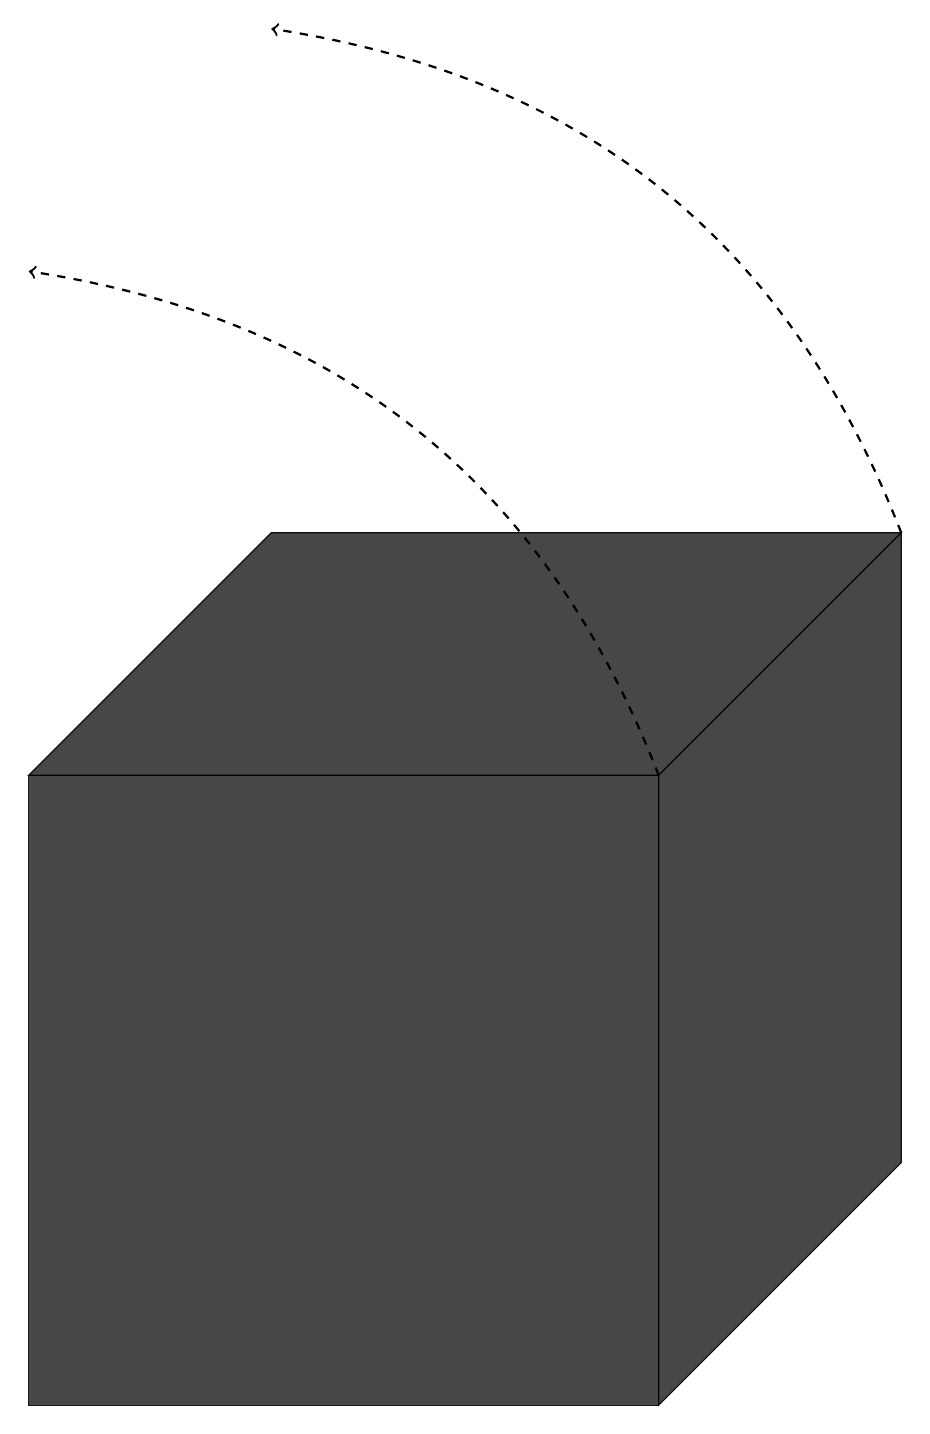
\begin{tikzpicture}
\coordinate (O) at (0,0,0);
\coordinate (A) at (0,\Width,0);
\coordinate (B) at (0,\Width,\Height);
\coordinate (C) at (0,0,\Height);
\coordinate (D) at (\Depth,0,0);
\coordinate (E) at (\Depth,\Width,0);
\coordinate (F) at (\Depth,\Width,\Height);
\coordinate (G) at (\Depth,0,\Height);
\coordinate (X) at (0,\Height * 1.8,0);
\coordinate (Z) at (0,\Height * 1.8,\Depth);

%\draw[blue,fill=black!10] (O) -- (C) -- (G) -- (D) -- cycle;% Bottom Face
%\draw[blue,fill=black!10] (O) -- (A) -- (E) -- (D) -- cycle;% Back Face
%\draw[blue,fill=black!10] (O) -- (A) -- (B) -- (C) -- cycle;% Left Face
\draw[black,fill=black!80,opacity=0.9] (D) -- (E) -- (F) -- (G) -- cycle;% Right Face
\draw[black,fill=black!80,opacity=0.9] (C) -- (B) -- (F) -- (G) -- cycle;% Front Face
\draw[black,fill=black!80,opacity=0.9] (A) -- (B) -- (F) -- (E) -- cycle;% Top Face
\draw [line width=20pt, thick, dashed, ->] (E) to [bend right = 30] (X);
\draw [thick,dashed, ->] (F) to [bend right = 30] (Z);
%% Following is for debugging purposes so you can see where the points are
%% These are last so that they show up on top
%\foreach \xy in {O, A, B, C, D, E, F, G}{
%    \node at (\xy) {\xy};
%}
\end{tikzpicture}


\end{document}